% Provenance (never printed): see sources/outline_sources.md (Year 1: solute and particle
% fluxes; the Hjulstrom diagram; settling velocity; denudation rates). Exercise and problem
% values in the Book 3 scratch calculator calc/ch20.py; figure data from
% figdata/bachelor-1/settling.py and threshold.py. Erosion, transport and deposition are
% Book 1's (g5); the sediment load in three forms, the denudation rate and isostatic rebound
% are Book 2's (g12), re-founded here (load, denudation rate) or recalled (rebound); discharge
% and the drainage basin are Book 2 g10's; Airy isostasy is ch. 11's; viscosity, Stokes' law
% and the Reynolds number are the physics books' (admitted, pointer). Grain-size classes and
% sorting belong to ch. 21.
\chapter{अपरदन और परिवहन}\label{ch:b1:erosion-transport}

एक तूफ़ान के बाद पुल के नीचे की नदी भूरी बहती है। जो पानी एक दिन पहले साफ़ था वह कीचड़ से गाढ़ा है, खंभों के चारों ओर भँवर बनाता है और टहनियाँ बहाता है, और तल पर, अनदेखे, लुढ़कते समय कंकड़ एक-दूसरे से टकराते हैं। हर सेकंड बाढ़ ज़मीन के टन भर बहा ले जाती है। नीचे की ओर, एक बाँध के पीछे, वही कीचड़ जलाशय के स्थिर पानी में बैठता है, जो हर वर्ष अपने आयतन का थोड़ा खोता है; और भी आगे, नदी के मुहाने पर, वह समुद्र में एक भूरे पंख की तरह फैलता है जो अंतरिक्ष से दिखाई दे सकता है। यह अध्याय उस यात्रा में संख्याएँ रखता है: नदी कितना और किन रूपों में ढोती है, एक कण कितनी तेज़ी से डूबता है, उसे चलाने के लिए कितनी धारा चाहिए, और अंततः पूरा भूदृश्य कितनी तेज़ी से घिसता है।

\begin{recall}
अपरदन भूमि का घिसना और उसके टुकड़ों का बहाना है; निक्षेपण उनका वहाँ बिछना है जहाँ वाहक धीमा होता है (पुस्तक~1, कक्षा~5)। एक नदी अपना तलछट-भार \omterm{def:b1:erosion-transport:load}{तल-भार}, \omterm{def:b1:erosion-transport:load}{निलंबित भार} और \omterm{def:b1:erosion-transport:load}{घुला भार} के रूप में ढोती है; किसी क्षेत्र की \omterm{def:b1:erosion-transport:denudation}{अपक्षरण-दर} उससे प्रति इकाई समय हटी चट्टान की मोटाई है, मीटर प्रति दस लाख वर्ष में; जब अपरदन \omterm{def:b1:layered-earth:layers}{भूपर्पटी} की एक मोटाई $e$ हटाता है, तो समस्थानिक प्रत्यावर्तन सतह को केवल $e(1 - \rho_c/\rho_m)$ नीचे जाने देता है (पुस्तक~2, कक्षा~12)। नदी का निस्सरण वह जल-आयतन है जो प्रति इकाई समय एक अनुप्रस्थ काट से गुज़रता है, और उसका जल-विभाजक वह क्षेत्र जो उसे आपूर्ति करता है (पुस्तक~2, कक्षा~10)। एरी \omterm{def:b1:isostasy-gravity:isostasy}{समस्थिति} में \omterm{def:b1:layered-earth:layers}{भूपर्पटी} अपने उच्चावच के समानुपाती जड़ के साथ मेंटल पर तैरती है (\cref{prop:b1:isostasy-gravity:airy})। सिलिकेटों का \omterm{def:b1:weathering-clays:hydrolysis}{जल-अपघटन} आयन और घुली सिलिका नदियों को देता है (\cref{def:b1:weathering-clays:hydrolysis})। किसी तरल की गतिक श्यानता $\mu$ उसके कर्तन के प्रतिरोध को मापती है, और गतिज श्यानता $\nu = \mu/\rho$ है; व्यास $d$ का एक गोला, धीमे वेग $w$ से किसी तरल में चलता हुआ, $3\pi\mu d w$ का अवरोध अनुभव करता है (स्टोक्स का नियम); रेनॉल्ड्स संख्या $w d/\nu$ जड़त्व की तुलना श्यान बलों से करती है, और गोले के चारों ओर प्रवाह तब तक चिकना रहता है जब तक वह छोटा है (भौतिकी की पुस्तकें)।
\end{recall}

\section{घुले और कण-प्रवाह}\label{sec:b1:erosion-transport:fluxes}

एक नदी ज़मीन को दो तरीकों से हटाती है: घोल में पदार्थ के रूप में, जो \omterm{def:b1:weathering-clays:weathering}{रासायनिक अपक्षय} के उत्पाद हैं, और ठोस कणों के रूप में, जो \omterm{def:b1:weathering-clays:weathering}{भौतिक अपक्षय} के उत्पाद और \omterm{def:b1:weathering-clays:weathering}{रासायनिक अपक्षय} के अघुलनशील अवशेष हैं। दोनों अलग तरह से चलते हैं, और कण स्वयं भी दो तरीकों से चलते हैं।

\begin{definition}[घुला भार, निलंबित भार, तल-भार]\label{def:b1:erosion-transport:load}
एक नदी का भार वह पदार्थ है जो वह एक अनुप्रस्थ काट से आगे ले जाती है, तीन भागों में, जो इस पर भिन्न हैं कि वे कैसे चलते हैं। \emph{घुला भार}\index{घुला भार} घोल में पदार्थ है, आयन और घुली सिलिका, जो अपनी गति से जल के साथ चलता है। \emph{निलंबित भार}\index{निलंबित भार} प्रवाह के भीतर उसकी प्रक्षुब्धता द्वारा ऊपर थामे गए कणों से बना है, अधिकतर मृत्तिका, गाद और बारीक बालू, जो जल की गति के लगभग समान गति से चलते हैं और शायद ही तल को छूते हैं। \emph{तल-भार}\index{तल-भार} उन कणों से बना है जो तल के साथ लुढ़कते, खिसकते या उछलते हैं, उससे बार-बार \omterm{def:b1:geological-maps:geological-map}{संपर्क} में, जल से कहीं धीमे।
\end{definition}

\begin{omfigure}
\begin{tikzpicture}[font=\footnotesize, >={Stealth[length=4pt]}]
% schematic: the three loads of a river (side view) and the forces on a bed grain
\fill[omDef!12] (0,0) rectangle (9,3.2);
\draw[omDef!80!black, thick] (0,3.2) -- (9,3.2);
\node[anchor=south west, omDef!80!black] at (0,3.2) {जल की सतह};
% flow profile arrows (velocity grows upward)
\foreach \y/\l in {0.35/0.5, 0.8/0.9, 1.4/1.15, 2.1/1.3, 2.8/1.4} {\draw[->, black!55] (0.25,\y) -- ++(\l,0);}
\draw[black!55] (0.25,0.12) -- (0.25,3.05);
\node[anchor=north west, black!65, align=left] at (0.2,-0.15) {प्रवाह-वेग\\ परिच्छेद};
% bed
\fill[black!12] (0,-0.05) rectangle (9,0.12);
\foreach \x in {0.1,0.45,...,8.9} {\fill[black!45] (\x,0.0) circle[radius=0.09];}
% dissolved load: ions
\foreach \x/\y/\s in {2.3/2.7/+, 3.1/1.9/-, 4.0/2.85/+, 4.7/2.2/-, 5.6/2.75/+, 6.3/1.85/+, 7.2/2.6/-, 8.2/2.2/+, 2.7/1.2/-, 7.8/1.3/-} {\node[circle, draw=omThm, inner sep=0.2pt, minimum size=7pt, font=\tiny, text=omThm] at (\x,\y) {$\s$};}
% suspended load: fine grains, denser near the bed
\foreach \x/\y in {2.1/1.5, 2.6/0.9, 3.0/2.5, 3.4/0.6, 3.7/1.4, 4.2/0.8, 4.4/1.9, 4.9/0.55, 5.2/1.2, 5.5/2.1, 5.9/0.7, 6.1/1.5, 6.6/0.9, 6.9/2.3, 7.4/0.6, 7.6/1.7, 8.0/0.85, 8.5/1.4, 3.9/0.45, 5.0/0.35, 6.4/0.4, 2.4/0.45, 8.6/0.5} {\fill[brown!75!black] (\x,\y) circle[radius=0.05];}
% bed load: rolling and hopping grains
\fill[black!60] (3.2,0.27) circle[radius=0.15];
\draw[->, black!70] (3.0,0.55) arc[start angle=150, end angle=30, radius=0.25];
\fill[black!60] (5.6,0.25) circle[radius=0.12];
\draw[->, black!70, densely dashed] (4.6,0.2) .. controls (4.9,0.9) and (5.3,0.7) .. (5.55,0.4);
\fill[black!60] (4.6,0.22) circle[radius=0.06];
% labels
\node[omThm, anchor=west] at (9.2,2.5) {घुला भार: आयन};
\node[brown!75!black, anchor=west] at (9.2,1.5) {निलंबित भार:};
\node[brown!75!black, anchor=west] at (9.2,1.1) {मृत्तिका, गाद, बारीक बालू};
\node[black!75, anchor=west] at (9.2,0.4) {तल-भार: लुढ़कते,};
\node[black!75, anchor=west] at (9.2,0.0) {खिसकते, उछलते कण};
\draw[->, thick, black!70] (6.8,3.55) -- node[above] {प्रवाह} (8.6,3.55);
% inset: forces on a grain resting on two others; it pivots about its downstream contact
\begin{scope}[xshift=11.8cm, yshift=-2.2cm]
  \fill[black!12] (-1.2,-0.4) rectangle (1.2,0);
  \fill[black!40] (-0.6,-0.15) circle[radius=0.28]; \fill[black!40] (0.6,-0.15) circle[radius=0.28];
  \fill[black!65] (0,0.166) circle[radius=0.4];
  \draw[->, thick, omDef!80!black] (0,0.166) -- (0,1.15) node[above] {उत्थापन};
  \draw[->, thick, omThm] (0,0.166) -- (1.05,0.166) node[right] {कर्षण-बल};
  \draw[->, thick, black] (0,0.166) -- (0,-0.8) node[below] {जलमग्न भार};
  \draw[->, thick, black!60] (-1.4,0.85) -- (-0.5,0.85) node[pos=0, left] {प्रवाह};
  \fill[red!60!black] (0.353,-0.020) circle[radius=0.045];
  \node[font=\scriptsize, anchor=north west, black!70] at (0.5,-0.4) {धुरी};
\end{scope}
\end{tikzpicture}

{\small एक नदी के तीन भार, किनारे से देखे गए (योजनाबद्ध, पैमाने पर नहीं)। प्रवाह सतह के निकट सबसे तेज़ है और तल पर शून्य तक धीमा होता है। आयन पूरी गहराई में फैले हैं; निलंबित कण भँवरों द्वारा ढोए जाते हैं, उनमें से अधिक तल के निकट; \omterm{def:b1:erosion-transport:load}{तल-भार} के कण लुढ़कते, खिसकते या छोटी उछालें लेते हैं। दाएँ: तल के एक कण पर बल। प्रवाह का कर्षण और उत्थापन उसे अपने निचले प्रतिवेशी पर, संपर्क-बिंदु के चारों ओर, लुढ़काने का प्रयास करते हैं; पानी में उसका भार उसे रोकता है।}
\label{fig:b1:erosion-transport:loads}
\end{omfigure}

दो ठोस भारों के बीच की सीमा कण के आकार से तय नहीं होती: वह प्रवाह पर निर्भर है। एक बाढ़ जो बालू को निलंबन में ढोती है, घटने पर उसे तल पर, \omterm{def:b1:erosion-transport:load}{तल-भार} के रूप में, छोड़ देती है; इसके विपरीत सबसे बारीक मृत्तिका लगभग किसी भी धारा में निलंबन में रहती है और बहती नदी के तल पर शायद ही मिलती है। हर भार एक फ़्लक्स के रूप में मापा जाता है, नदी के एक अनुप्रस्थ काट से प्रति इकाई समय गुज़रता द्रव्यमान।

\begin{proposition}[एक भार का फ़्लक्स]\label{prop:b1:erosion-transport:flux}
मान लीजिए $c$ एक घुले या \omterm{def:b1:erosion-transport:load}{निलंबित भार} की सांद्रता है (जल के प्रति इकाई आयतन में द्रव्यमान) और $u$ जल का वेग, दोनों क्षेत्रफल $A$ की काट में फैले हुए। (1)~काट से गुज़रता भार का तात्कालिक फ़्लक्स है
\[
  F = \iint_A c\,u\,\mathrm dA = \overline{c}_Q\,Q,
\]
जहाँ $Q = \iint_A u\,\mathrm dA$ निस्सरण है और $\overline{c}_Q$ वेग से भारित माध्य सांद्रता। (2)~एक काल $T$ में, जिसमें नदी का निस्सरण $Q(t)$ और सांद्रता $C(t)$ बदलते हैं, ढोया गया द्रव्यमान है
\[
  M = \int_0^T Q\,C\,\mathrm dt = T\left(\overline{Q}\;\overline{C} +
  \operatorname{cov}(Q, C)\right),
\]
जहाँ पट्टियाँ समय पर माध्य हैं और $\operatorname{cov}(Q, C)$ $(Q - \overline{Q})(C - \overline{C})$ का माध्य है। माध्य निस्सरण और माध्य सांद्रता का गुणनफल सही द्रव्यमान तभी देता है जब दोनों असहसंबद्ध हों।
\end{proposition}

\begin{proof}
(1)~समय $\mathrm dt$ में एक छोटे क्षेत्रफल $\mathrm dA$ से होकर पार करता जल आयतन $u\,\mathrm dA\,\mathrm dt$ भरता है, जो द्रव्यमान $c\,u\,\mathrm dA\,\mathrm dt$ ढोता है; काट पर जोड़ने से $F$ मिलता है, और $\overline{c}_Q$ को $F/Q$ परिभाषित किया गया है। (2)~लिखिए $Q = \overline{Q} + Q'$ और $C =
\overline{C} + C'$, जहाँ उतार-चढ़ाव $Q'$ और $C'$ काल पर शून्य माध्य रखते हैं। तब $QC = \overline{Q}\,\overline{C} + \overline{Q}\,C' + Q'\,\overline{C}
+ Q'C'$; दो मध्य पद शून्य पर औसत होते हैं, और $Q'C'$ का माध्य सहप्रसरण है।
\end{proof}

सहप्रसरण \omterm{def:b1:erosion-transport:load}{निलंबित भार} के लिए मायने रखता है। बाढ़ों में उसकी सांद्रता तीव्र रूप से बढ़ती है, जब वर्षा मिट्टी को धाराओं में धोती है और तेज़ प्रवाह तल से कणों को उठाता है, इसलिए $Q$ और $C$ साथ-साथ बढ़ते हैं: एक नदी के वार्षिक तलछट का बड़ा भाग कुछ दिनों की बाढ़ में गुज़रता है, और एक नमूना-अभियान जो उन्हें चूक जाए, या माध्य सांद्रता को माध्य निस्सरण से गुणा करना, भार को कम आँकता है। \omterm{def:b1:erosion-transport:load}{घुला भार} उलटी तरह बर्ताव करता है: बाढ़ें उसे तनु करती हैं, और उसकी सांद्रता कम प्रवाह पर सबसे ऊँची होती है, जब नदी को भूजल से पोषण मिलता है जो चट्टान के साथ लंबे समय से \omterm{def:b1:geological-maps:geological-map}{संपर्क} में रहा है।

\begin{method}[गॉजिंग से नदी का वार्षिक भार]\label{met:b1:erosion-transport:gauging}
\begin{enumerate}
  \item एक गॉजिंग स्टेशन पर निस्सरण लगातार दर्ज कीजिए।
  \item कई निस्सरणों पर जल के नमूने लीजिए, बाढ़ें सहित, और तलछट का द्रव्यमान प्रति लीटर (छानकर और तौलकर) तथा हर घुली प्रजाति का मापिए।
  \item सांद्रताओं को नमूना-समय के निस्सरण से भारित कीजिए ताकि प्रवाह-भारित माध्य सांद्रता मिले, या सांद्रता को निस्सरण का फलन मानकर पूरे अभिलेख पर लागू कीजिए।
  \item वर्ष के कुल जल-आयतन से गुणा कीजिए, या अभिलेख पर $Q\,C\,\Delta
        t$ का योग कीजिए (\cref{prop:b1:erosion-transport:flux})।
  \item \omterm{def:b1:erosion-transport:load}{तल-भार} जोड़िए, जो जल-नमूनाकार चूक जाते हैं, अलग मापों से या एक अनुमानित भाग के रूप में।
  \item घुले भार के लिए, वह हटाइए जो चट्टान से नहीं आता: वर्षा द्वारा लाए लवण, और बाइकार्बोनेट के लिए वह कार्बन जो हवा से लिया गया (\cref{ch:b1:weathering-clays})।
\end{enumerate}
\end{method}

\begin{omfigure}
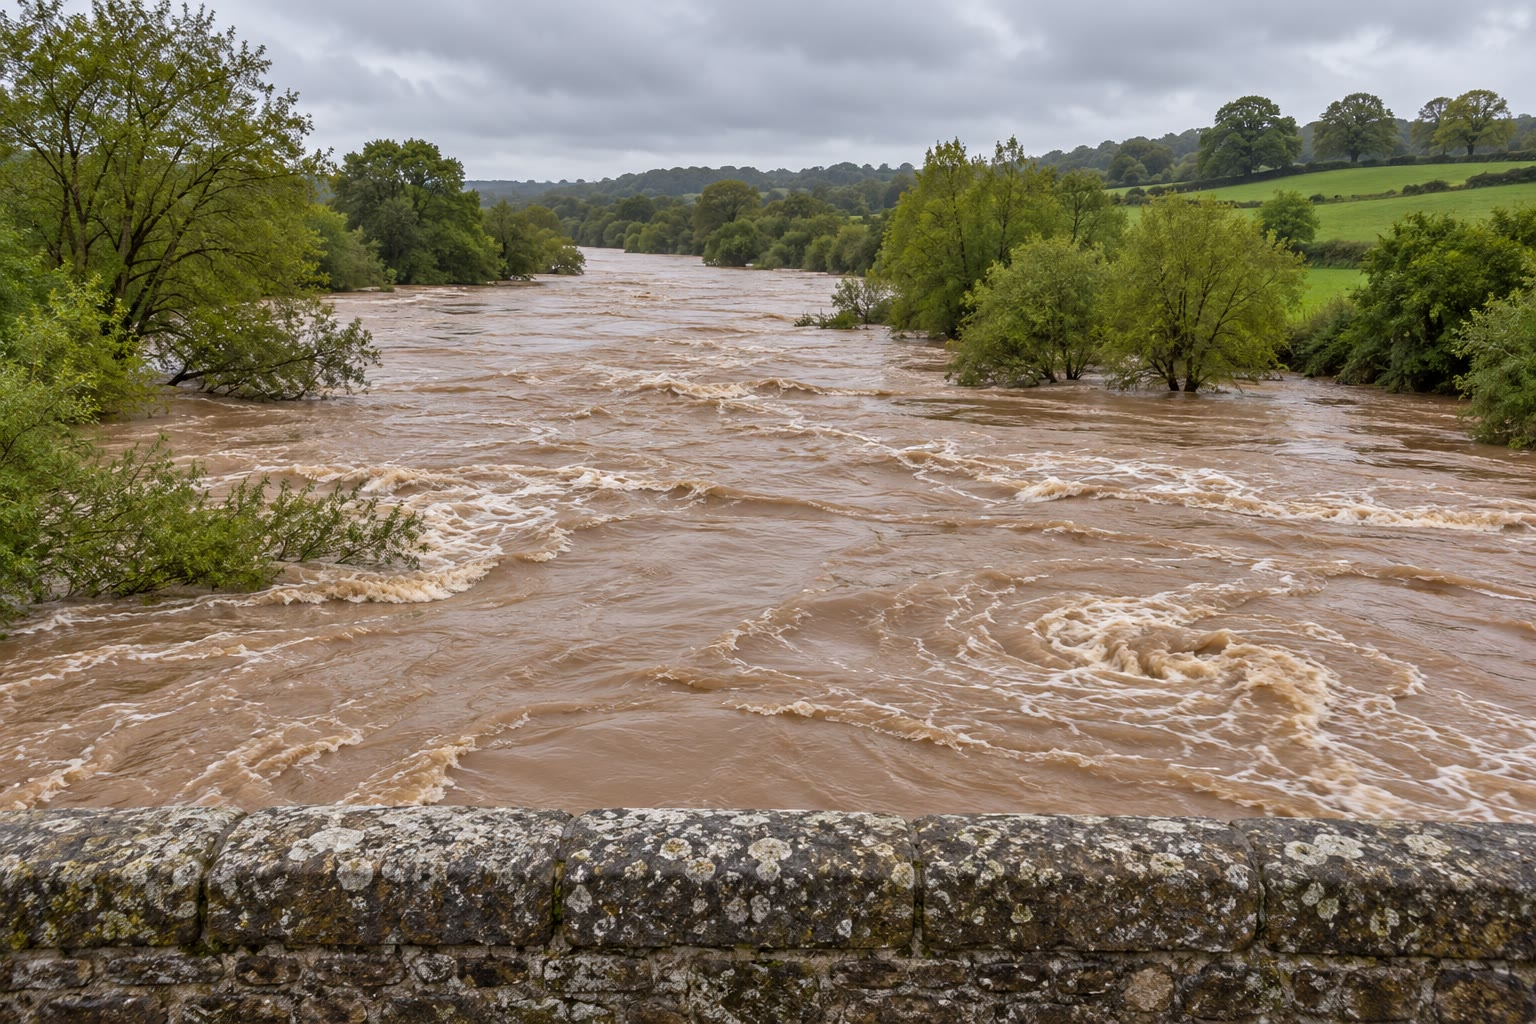
\includegraphics[height=5.1cm]{images/book3/ai/b1-muddy-river.jpg}\hfill
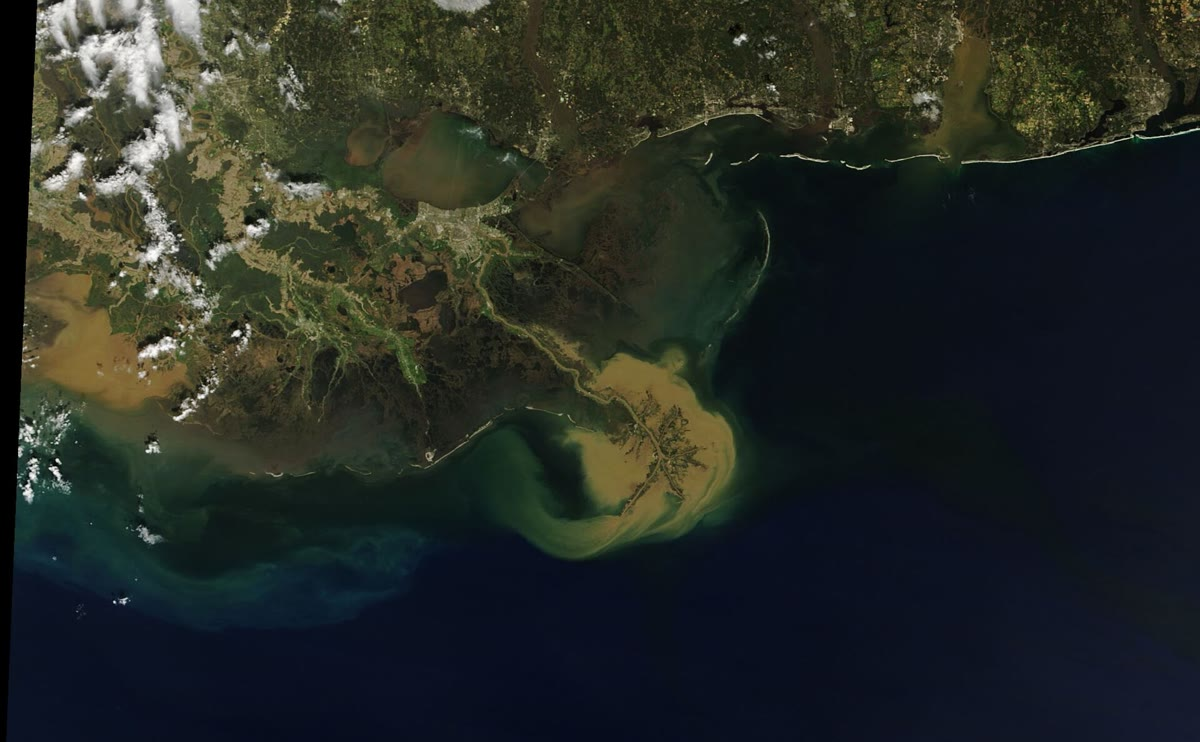
\includegraphics[height=5.1cm]{images/book3/b1-mississippi-plume.jpg}
{\small बाएँ: बाढ़ में एक नदी भूरा, तलछट से भरा पानी ढोती है (AI से बनाया गया चित्र)। दाएँ: मिसिसिपी का बाढ़-पंख, जो उसके डेल्टा के चारों ओर मेक्सिको की खाड़ी में उड़ेला जा रहा है, 4 मार्च 2018 को टेरा उपग्रह पर MODIS उपकरण से देखा गया; निलंबित कीचड़ समुद्र को भूरा और हरा रंगता है, और दक्षिण-पूर्वी हवा पंख को उत्तर-पश्चिम की ओर धकेलती है। चित्र: NASA Earth Observatory, Joshua Stevens द्वारा, सार्वजनिक क्षेत्र, विकिमीडिया कॉमन्स के माध्यम से।}
\label{fig:b1:erosion-transport:plume}
\end{omfigure}
% ledger: commons:mississippi-plume

\emph{विश्व की नदियाँ।} मानवीय प्रभाव से पहले, विश्व की नदियाँ लगभग \qty{14}{Gt} निलंबित तलछट प्रति वर्ष तटीय महासागर को ले जाती थीं, \omterm{def:b1:erosion-transport:load}{तल-भार} के साथ \qty{15.5}{Gt}। लोगों ने यात्रा के दोनों सिरे बदल दिए हैं: खेती और वनों की कटाई ने मृदा-अपरदन बढ़ाया है, नदियों में लगभग \qty{2.3}{Gt} प्रति वर्ष जोड़ते हुए, जबकि जलाशय तलछट रोकते हैं: बड़े जलाशय लगभग \qty{20}{\percent} प्रवाह को फँसाते हैं और छोटे एक अन्य \qty{6}{\percent} को, और \qty{100}{Gt} से अधिक तलछट अब उन बाँधों के पीछे पड़ा है जो अधिकतर पिछले पचास वर्षों में बने। शुद्ध प्रभाव एक कमी है: आधुनिक प्रवाह लगभग \qty{12.6}{Gt} प्रति वर्ष है।
% ledger: syvitski:flux

\begin{dated}{2005}
निलंबित तलछट प्रवाह के आँकड़े, मानवीय प्रभाव से पहले और बाद के, 2005 में प्रकाशित नदी-तलछट के एक वैश्विक प्रतिरूप से आते हैं। उसके बाद से बाँध बने हैं।
\end{dated}
% ledger: syvitski:flux

\omterm{def:b1:erosion-transport:load}{घुला भार} छोटा है। 1963 में किए गए नदी-विश्लेषणों के एक क्लासिक संकलन ने विश्व की नदियों द्वारा समुद्र तक पहुँचाए घुले पदार्थ को लगभग \qty{3.9}{Gt} प्रति वर्ष पर रखा, आधुनिक निलंबित प्रवाह के लगभग \qty{30}{\percent}, \qty{120}{mg} प्रति लीटर के माध्य सांद्रता पर। बाइकार्बोनेट उसका लगभग आधा है, \qty{58}{mg.L^{-1}}, उसके बाद कैल्शियम, सिलिका, सल्फ़ेट, क्लोराइड और सोडियम। उसका एक भाग चट्टान से नहीं आता: बाइकार्बोनेट का बहुत-सा भाग हवा या मिट्टी से लिया कार्बन ढोता है, और क्लोराइड तथा सोडियम का एक भाग वर्षा द्वारा लाए समुद्री लवण से है। अलग-अलग नदियाँ इन माध्यों के चारों ओर व्यापक रूप से फैली हैं।
% ledger: livingstone:world-dissolved, syvitski:flux

\emph{एक द्रोणी का तलछट-बजट।} जल-विभाजक में अपरदित हर कण अपने निर्गम तक नहीं पहुँचता। किसी खेत से धुली मिट्टी ढलान के पैर पर रुक सकती है, बालू बाढ़-मैदान और नदी की रेतीली पट्टियों में सदियों तक जमा रह सकती है, और एक जलाशय उसमें आने वाले अधिकांश को रोक सकता है। निर्गम पर मापा गया भार इस बजट का संतुलन है: ढलानों और किनारों से जो अपरदित हुआ, उसमें से वह घटाकर जो रास्ते में संचित हुआ, और उसमें जोड़कर जो पुराने भंडारों से वापस लिया गया। गॉजिंग के कुछ दशकों में यह संतुलन दीर्घकालिक अपरदन-दर से किसी भी दिशा में बहुत दूर हो सकता है, और यही एक कारण है कि \cref{sec:b1:erosion-transport:denudation} की अन्य विधियाँ हैं।

\section{अवसादन-वेग}\label{sec:b1:erosion-transport:settling}

एक कण जल से घना है और डूबता है। क्या एक नदी उसे ढो सकती है, और वह कहाँ निक्षेपित होगा, यह पहले इस पर निर्भर है कि वह कितनी तेज़ी से डूबता है।

\begin{definition}[अवसादन-वेग]\label{def:b1:erosion-transport:settling}
एक कण का \emph{अवसादन-वेग}\index{अवसादन-वेग} $w_s$ वह स्थिर वेग है जिससे वह स्थिर जल में गिरता है, जब जल का अवरोध उसके जलमग्न भार, यानी उसके भार में से उस जल के उत्प्लावन को घटाकर जिसे वह विस्थापित करता है, के बराबर हो।
\end{definition}

स्थिर जल में छोड़ा गया कण तब तक त्वरित होता है जब तक उसका अवरोध, जो उसकी गति के साथ बढ़ता है, उसके जलमग्न भार के बराबर न हो जाए; एक बालू या गाद के कण के लिए यह एक सेकंड के छोटे अंश में होता है, इसलिए \omterm{def:b1:erosion-transport:settling}{अवसादन-वेग} वह गति है जिससे वह लगभग पूरी दूरी तक गिरता है। कण का घनत्व $\rho_s$ और जल का $\rho$ लेकर, सापेक्ष जलमग्न घनत्व के लिए $R = (\rho_s - \rho)/\rho$ लिखिए।

\begin{proposition}[स्टोक्स अवसादन]\label{prop:b1:erosion-transport:stokes}
व्यास $d$ और घनत्व $\rho_s$ का एक गोला, घनत्व $\rho$ और गतिक श्यानता $\mu$ वाले जल में धीरे गिरता हुआ, स्टोक्स के नियम के अंतर्गत, \omterm{def:b1:erosion-transport:settling}{अवसादन-वेग} रखता है
\[
  w_s = \frac{(\rho_s - \rho)\,g\,d^2}{18\,\mu} = \frac{R\,g\,d^2}{18\,\nu}.
\]
यह नियम तब तक लागू है जब तक कण की रेनॉल्ड्स संख्या $w_s d/\nu$ लगभग 1 से नीचे है, अर्थात व्यासों के लिए जो $d_1 = \left(18\,\nu^2/(R\,g)\right)^{1/3}$ से छोटे हैं।
\end{proposition}

\begin{proof}
गोले का भार $\rho_s g\,\pi d^3/6$ और उत्प्लावन $\rho g\,\pi d^3/6$ है, इसलिए उसका जलमग्न भार $(\rho_s - \rho)\,g\,\pi d^3/6$ है। \omterm{def:b1:erosion-transport:settling}{अवसादन-वेग} पर वह अवरोध $3\pi\mu d\,w_s$ के बराबर है:
\[
  (\rho_s - \rho)\,g\,\frac{\pi d^3}{6} = 3\pi\mu d\,w_s
  \quad\Longrightarrow\quad
  w_s = \frac{(\rho_s - \rho)\,g\,d^2}{18\,\mu},
\]
और अंश और हर को $\rho$ से भाग देने पर दूसरा रूप मिलता है। इस वेग पर रेनॉल्ड्स संख्या $R g d^3/(18\nu^2)$ है, जो $d = d_1$ पर 1 के बराबर है और $d^3$ के साथ बढ़ती है।
\end{proof}

घनत्व \qty{2650}{kg.m^{-3}} के क्वार्ट्ज हेतु, \qty{20}{\celsius} पर जल में, जिसका घनत्व \qty{998.2}{kg.m^{-3}} और श्यानता \qty{1.0016}{mPa.s} है: $R =
1.65$, $\nu = \qty{1.003e-6}{m^2.s^{-1}}$, और $g =
\qty{9.81}{m.s^{-2}}$ सहित सीमा $d_1 = \qty{0.104}{mm}$ है, एक बारीक बालू। इससे नीचे, स्टोक्स का नियम गाद और मृत्तिका के \omterm{def:b1:erosion-transport:settling}{अवसादन-वेग} देता है: \qty{10}{\micro m} आर-पार की एक गाद का कण \qty{9.0e-5}{m.s^{-1}} पर डूबता है, \qty{1}{m} लगभग तीन घंटों में; \qty{2}{\micro m} की एक मृत्तिका-कण \qty{3.6e-6}{m.s^{-1}} पर, \qty{1}{m} \num{3.2}~दिनों में। प्राकृतिक मृत्तिका-कण गोले नहीं, पत्र होते हैं, और भी धीरे डूबते हैं। \qty{5}{m} गहरा, पूर्णतः स्थिर जल ऐसी मृत्तिका से साफ़ होने में सोलह दिन लेगा; एक बहती नदी, जिसके भँवर उसे लगातार हिलाते रहते हैं, कभी साफ़ नहीं होती, इसीलिए सबसे बारीक कीचड़ समुद्र तक जाता है।
% ledger: hom:quartz, nist:water, const:gn

$d_1$ से ऊपर अवरोध वेग के अनुपात से अधिक तेज़ी से बढ़ता है: कण के पीछे बहता जल एक पीछे की धारा (वेक) में अलग हो जाता है, और बड़ी रेनॉल्ड्स संख्याओं पर अवरोध वेग के वर्ग के समानुपाती होता है। प्राकृतिक कणों पर प्रयोग एक ही सूत्र में समेटे गए हैं जो दोनों शासनों को जोड़ता है।

\begin{proposition}[संयुक्त अवसादन-नियम]\label{prop:b1:erosion-transport:combined}
छलनी-व्यास $d$ के प्राकृतिक कणों का \omterm{def:b1:erosion-transport:settling}{अवसादन-वेग}, सभी आकारों के लिए,
\[
  w_s = \frac{R\,g\,d^2}{C_1\,\nu + \sqrt{0.75\,C_2\,R\,g\,d^3}},
\]
जहाँ $C_1 = 18$ और $C_2 = 1.0$।
\end{proposition}
\admitted
% ledger: fc:settling

यह नियम फ़र्गसन और चर्च का है, जिन्होंने उसे प्राकृतिक बालू के मापे अवसादन-वेगों पर आरोपित किया। छोटे कणों के लिए वर्गमूल नगण्य है और वह स्टोक्स के नियम में घट जाता है; बड़े कणों के लिए हर का पहला पद नगण्य है और $w_s \to \sqrt{4 R g d/(3 C_2)}$, जो आकार के केवल वर्गमूल के साथ बढ़ता है। स्थिरांक कणों के आकार पर निर्भर हैं: $C_2 = 0.4$ चिकने गोलों का वर्णन करता है, बड़े मान अधिक कोणीय कणों का, जो अधिक अवरोध से मिलते हैं। दो नियम \qty{0.1}{mm} से ऊपर अलग होते हैं। \qty{1}{mm} के एक कण के लिए संयुक्त नियम \qty{0.126}{m.s^{-1}} देता है, स्टोक्स के नियम से सात गुना कम; \qty{10}{mm} के एक कंकड़ के लिए, \qty{0.46}{m.s^{-1}} के मुकाबले एक निरर्थक \qty{90}{m.s^{-1}} (नीचे का आरेख)।
% ledger: fc:settling

\begin{omfigure}
\begin{tikzpicture}[font=\small]
% settling velocity of quartz grains in water at 20 C (figdata/bachelor-1/settling.py)
\begin{axis}[width=11cm, xmode=log, ymode=log, xmin=0.001, xmax=10, ymin=1e-8, ymax=10, height=8cm,
    xlabel={कण का व्यास $d$ (\si{mm})}, ylabel={अवसादन-वेग (\si{m.s^{-1}})},
    ytick={1e-8,1e-6,1e-4,1e-2,1},
    legend style={at={(0.03,0.97)}, anchor=north west, font=\footnotesize}, legend cell align=left,
    grid=major, grid style={black!10}]
  \addplot[omDef, thick, dashed] table[x=d_mm, y=w_stokes] {figdata/out/bachelor-1-settling-curves.dat};
  \addplot[omThm, very thick] table[x=d_mm, y=w_fc] {figdata/out/bachelor-1-settling-curves.dat};
  \legend{स्टोक्स का नियम, संयुक्त नियम (प्राकृतिक कण)}
  \draw[black!55, densely dotted] (axis cs:0.1037,1e-7) -- (axis cs:0.1037,10);
  \node[font=\scriptsize, anchor=west, align=left, black!75] at (axis cs:0.115,1e-6) {कण रेनॉल्ड्स\\ संख्या $= 1$};
  \node[font=\scriptsize, black!70] at (axis cs:0.002,3e-8) {मृत्तिका};
  \node[font=\scriptsize, black!70] at (axis cs:0.016,3e-8) {गाद};
  \node[font=\scriptsize, black!70] at (axis cs:0.35,3e-8) {बालू};
  \node[font=\scriptsize, black!70] at (axis cs:4.5,3e-8) {बजरी};
  \draw[black!40] (axis cs:0.0039,1e-8) -- (axis cs:0.0039,1e-7);
  \draw[black!40] (axis cs:0.0625,1e-8) -- (axis cs:0.0625,1e-7);
  \draw[black!40] (axis cs:2,1e-8) -- (axis cs:2,1e-7);
\end{axis}
\end{tikzpicture}

{\small \qty{20}{\celsius} पर जल में क्वार्ट्ज के कणों का \omterm{def:b1:erosion-transport:settling}{अवसादन-वेग}, उनके व्यास के विरुद्ध, दोनों लघुगणकीय पैमानों पर: स्टोक्स का नियम और प्राकृतिक कणों का संयुक्त नियम, परिकलित। इन पैमानों पर स्टोक्स का नियम ढाल 2 की एक सीधी रेखा है। दोनों गाद और मृत्तिका के लिए मेल खाते हैं; लगभग \qty{0.1}{mm} से ऊपर, जहाँ कण रेनॉल्ड्स संख्या 1 पार करती है, पीछे की धारा का अवरोध मोटे कणों को धीमा करता है। तल पर के निशान कण-आकार वर्गों की सीमाएँ दिखाते हैं, \qty{3.9}{\micro m} ($1/256$~mm), \qty{62.5}{\micro m} ($1/16$~mm) और \qty{2}{mm} पर।}
\label{fig:b1:erosion-transport:settling}
\end{omfigure}
% ledger: fc:settling, usgs:wentworth-phi

बारीकतम मृत्तिका से लेकर मोटे बजरी तक, आरेख की परास में, \omterm{def:b1:erosion-transport:settling}{अवसादन-वेग} आठ परिमाण-कोटियों तक फैलता है। यही पहला कारण है कि नदियाँ अपने तलछट को छाँटती हैं: धीमा होता प्रवाह अपनी बजरी तुरंत गिरा देता है, अपनी बालू मीटरों के भीतर, अपनी गाद किलोमीटरों के भीतर, और अपनी मृत्तिका को किसी झील या समुद्र तक ले जाता है। कण-आकार वर्ग और तलछट का छँटाव अगले अध्याय का विषय हैं (\cref{ch:b1:clastic-sediments})।

\section{गति की देहली और हियुलस्ट्रॉम आरेख}\label{sec:b1:erosion-transport:threshold}

तल पर विश्राम में एक कण को, नदी के उसके ऊपर बहते जल का बल गति में डालता है। वह बल एक प्रतिबल से मापा जाता है।

\begin{definition}[तल कर्तन-प्रतिबल, कर्तन-वेग]\label{def:b1:erosion-transport:bed-shear}
एक प्रवाह का \emph{तल कर्तन-प्रतिबल}\index{तल कर्तन-प्रतिबल} $\tau_b$ वह बल है जो वह अपने तल पर, तल के समांतर, प्रवाह की दिशा में, प्रति इकाई क्षेत्रफल लगाता है। कर्तन-वेग $u_* = \sqrt{\tau_b/\rho}$ है, एक वेग जो उसी प्रतिबल को मापता है।
\end{definition}

\omterm{def:b1:erosion-transport:bed-shear}{तल कर्तन-प्रतिबल} धारा-मापी से नहीं पढ़ा जा सकता, परंतु एक स्थिर प्रवाह में वह बलों के संतुलन से निकलता है।

\begin{proposition}[गहराई-ढाल गुणनफल]\label{prop:b1:erosion-transport:depth-slope}
गहराई $h$ के एक स्थिर, एकसमान प्रवाह में, छोटे ढाल $S$ वाली एक चौड़ी नहर में, \omterm{def:b1:erosion-transport:bed-shear}{तल कर्तन-प्रतिबल} है
\[
  \tau_b = \rho\,g\,h\,S .
\]
\end{proposition}

\begin{proof}
एक नहर-खंड के ऊपर का जल जिसकी लंबाई प्रवाह के अनुदिश $L$ और इकाई चौड़ाई है, विचार कीजिए, नहर इतनी चौड़ी है कि उसके किनारों को नज़रअंदाज़ किया जा सकता है। प्रवाह स्थिर और एकसमान है, इसलिए यह जल त्वरित नहीं होता और उस पर के बल संतुलित हैं। उसके ऊपरी-प्रवाह और निचले-प्रवाह फलकों पर दाब-बल समान और विपरीत हैं, क्योंकि दोनों पर गहराई एक ही है। प्रवाह के अनुदिश भार का घटक $\rho g h L \sin\beta$ शेष रहता है, जहाँ $\beta$ तल का कोण है, और तल का घर्षण $\tau_b L$, उसके विरुद्ध। अतः $\tau_b
= \rho g h \sin\beta$, और एक छोटे कोण के लिए $\sin\beta \approx \tan\beta = S$।
\end{proof}

\qty{2}{m} गहरी एक नदी, \num{0.001} ढाल पर, यानी प्रति किलोमीटर एक मीटर गिरावट, के लिए $\tau_b = 998.2 \times 9.81 \times 2 \times 0.001 =
\qty{19.6}{Pa}$ है, और कर्तन-वेग \qty{0.140}{m.s^{-1}}। एक ऐसी नहर में जो चौड़ी नहीं है, किनारे घर्षण का अपना भाग लेते हैं, और गहराई को जल-त्रिज्या से बदला जाता है, काट का क्षेत्रफल उसकी गीली परिधि से भाग देने पर (\cref{exo:b1:erosion-transport:5})।

\emph{कण पर बल।} प्रवाह एक तल के कण को अपने कर्षण से धकेलता है और अपने ऊपर के तेज़ प्रवाह से उठाता है (इस अध्याय के पहले चित्र का अंतःचित्र)। दोनों बल कण के क्षेत्रफल पर कार्य करते हैं, इसलिए वे $\tau_b
d^2$ के साथ मापे जाते हैं; कण अपने जलमग्न भार से विरोध करता है, जो $(\rho_s - \rho) g d^3$ के साथ मापा जाता है। दोनों का अनुपात दिए गए कण के लिए प्रवाह की शक्ति का स्वाभाविक माप है।

\begin{definition}[शील्ड्स प्राचल, गति की देहली]\label{def:b1:erosion-transport:threshold}
\omterm{def:b1:erosion-transport:bed-shear}{तल कर्तन-प्रतिबल} $\tau_b$ वाले प्रवाह का, व्यास $d$ और घनत्व $\rho_s$ के कणों पर, \emph{शील्ड्स प्राचल}\index{शील्ड्स प्राचल} है
\[
  \theta = \frac{\tau_b}{(\rho_s - \rho)\,g\,d}.
\]
कणों की \emph{गति की देहली}\index{गति की देहली} \omterm{def:b1:erosion-transport:bed-shear}{तल कर्तन-प्रतिबल} है, या शील्ड्स प्राचल का मान $\theta_c$, जिस पर वे चलने लगते हैं।
\end{definition}
% ledger: hecras:thresholds

क्रांतिक मान $\theta_c$ नहरों (फ़्लूम) में मापा जाता है, और माप जब एक विमाहीन कण-आकार के विरुद्ध आलेखित होते हैं जो कण और तरल दोनों को मिलाता है, तब एक ही वक्र पर गिरते हैं।

\begin{proposition}[सॉल्सबी और व्हाइटहाउस का देहली-वक्र]\label{prop:b1:erosion-transport:soulsby}
एक समतल तल पर व्यास $d$ के कणों के लिए, $D_* = d\,\left(R\,g/\nu^2\right)^{1/3}$ के साथ, क्रांतिक \omterm{def:b1:erosion-transport:threshold}{शील्ड्स प्राचल} है
\[
  \theta_c = \frac{0.3}{1 + 1.2\,D_*} + 0.055\left(1 - e^{-0.02\,D_*}\right),
\]
और क्रांतिक \omterm{def:b1:erosion-transport:bed-shear}{तल कर्तन-प्रतिबल} $\tau_c = \theta_c\,(\rho_s - \rho)\,g\,d$ है।
\end{proposition}
\admitted
% ledger: hecras:thresholds

मोटे कणों के लिए $\theta_c$ \num{0.055} की ओर जाता है: बजरी तब चलती है जब \omterm{def:b1:erosion-transport:bed-shear}{तल कर्तन-प्रतिबल}, प्रति इकाई क्षेत्रफल, एक व्यास मोटी कणों की परत के जलमग्न भार के लगभग बीसवें भाग तक पहुँचता है। स्थिर देहली का उपयोग करने वाले तलछट-परिवहन के सूत्र \num{0.03} से \num{0.047} तक के मान लेते हैं, उनमें से अंतिम मेयर-पीटर और मूलर के क्लासिक \omterm{def:b1:erosion-transport:load}{तल-भार} सूत्र में। बारीक बालू के लिए $\theta_c$ फिर बढ़ता है, \qty{0.1}{mm} पर \num{0.077} तक: छोटे कण तल के निकट पानी की धीमी, श्यान परत में पड़ते हैं और अपने पड़ोसियों से आच्छादित रहते हैं। न्यूनतम, \num{0.030}, लगभग \qty{0.7}{mm} पर गिरता है। पास्कल में देहली सदा आकार के साथ बढ़ती है (नीचे का आरेख): \qty{0.1}{mm} की बालू के लिए \qty{0.13}{Pa}, \qty{1}{mm} पर \qty{0.51}{Pa}, \qty{10}{mm} पर \qty{9.0}{Pa}, \qty{64}{mm} के एक पत्थर के लिए \qty{57}{Pa}।
% ledger: hecras:thresholds

\begin{omfigure}
\begin{tikzpicture}[font=\small]
% threshold of motion of quartz grains in water at 20 C (figdata/bachelor-1/threshold.py, Soulsby and Whitehouse)
\begin{axis}[name=a, width=6.9cm, height=6cm, xmode=log, xmin=0.0625, xmax=100, ymin=0, ymax=0.12,
    xlabel={कण का व्यास $d$ (\si{mm})}, ylabel={क्रांतिक शील्ड्स प्राचल $\theta_c$},
    yticklabel style={/pgf/number format/fixed, /pgf/number format/precision=2},
    grid=major, grid style={black!10}, title={\footnotesize (क) विमाहीन}]
  \addplot[omThm, very thick] table[x=d_mm, y=theta] {figdata/out/bachelor-1-threshold-shields.dat};
  \draw[black!50, dashed] (axis cs:0.0625,0.055) -- (axis cs:100,0.055) node[pos=0.7, above, font=\scriptsize, black!70] {$0.055$};
\end{axis}
\begin{axis}[at={(a.east)}, anchor=west, xshift=2.0cm, width=6.9cm, height=6cm, xmode=log, ymode=log,
    xmin=0.0625, xmax=100, ymin=0.05, ymax=200,
    xlabel={कण का व्यास $d$ (\si{mm})}, ylabel={क्रांतिक तल कर्तन-प्रतिबल $\tau_c$ (\si{Pa})},
    grid=major, grid style={black!10}, title={\footnotesize (ख) पास्कल में}]
  \addplot[omDef, very thick] table[x=d_mm, y=tau_cr] {figdata/out/bachelor-1-threshold-shields.dat};
\end{axis}
\end{tikzpicture}

{\small \qty{20}{\celsius} पर जल में क्वार्ट्ज के कणों की \omterm{def:b1:erosion-transport:threshold}{गति की देहली}, सॉल्सबी और व्हाइटहाउस के वक्र से, बारीक-बालू की सीमा (\qty{0.0625}{mm}) से एक पत्थर के आकार तक परिकलित। (क)~क्रांतिक \omterm{def:b1:erosion-transport:threshold}{शील्ड्स प्राचल} बजरी के लिए लगभग स्थिर है और बारीक बालू के लिए बढ़ता है। (ख)~क्रांतिक \omterm{def:b1:erosion-transport:bed-shear}{तल कर्तन-प्रतिबल} बजरी के लिए लगभग व्यास के अनुपात में बढ़ता है।}
\label{fig:b1:erosion-transport:threshold}
\end{omfigure}
% ledger: hecras:thresholds

\begin{example}[नदी क्या हिलाती है]\label{ex:b1:erosion-transport:river}
\qty{2}{m} गहरी, \num{0.001} ढाल वाली नदी में $\tau_b =
\qty{19.6}{Pa}$। \qty{20}{mm} के कणों के लिए, $\theta = 19.6/(1651.8 \times
9.81 \times 0.020) = 0.060$, अपनी देहली \num{0.055} से ठीक ऊपर: वे चलते हैं। \qty{40}{mm} के कणों के लिए, $\theta = 0.030$, देहली का आधा: वे रुकते हैं। नदी अपने तल को मोटी बजरी तक हिलाती है; \qty{1}{mm} की बालू के लिए, $\theta = 1.21$, \num{0.031} की देहली से लगभग चालीस गुना।
\end{example}

\emph{निलंबन में।} एक बार गतिमान, एक कण तल के साथ उछलता है या प्रवाह में उठा लिया जाता है, इस पर निर्भर करते हुए कि क्या भँवर, जिनकी गति कर्तन-वेग की कोटि की है, उसे उसके अवसादन के विरुद्ध ऊपर थाम सकते हैं।

\begin{proposition}[निलंबन का मानदंड]
\label{prop:b1:erosion-transport:suspension}
एक \omterm{def:b1:erosion-transport:settling}{अवसादन-वेग} $w_s$ वाला कण एक प्रक्षुब्ध प्रवाह में निलंबन में तभी रह सकता है जब कुछ भँवर उसके डूबने से तेज़ ऊपर उठें। भँवरों के ऊर्ध्वगामी वेग कर्तन-वेग $u_*$ की कोटि के हैं, इसलिए निलंबन तब शुरू होता है जब $u_*$, $w_s$ के निकट आता है, और तब पूरी तरह विकसित होता है जब $u_*$ उससे अधिक हो; यह अध्याय $u_* = w_s$ को निलंबन की सीमा लेता है।
\end{proposition}
\admitted
% ledger: bagnold:suspension

उदाहरण की नदी में $u_* = \qty{0.140}{m.s^{-1}}$ है, जिसे अवसादन का संयुक्त नियम \qty{1.16}{mm} के कणों को देता है: लगभग एक मिलीमीटर से बारीक बालू निलंबन में चलती है, मोटी बालू और बजरी \omterm{def:b1:erosion-transport:load}{तल-भार} के रूप में। तर्क बैगनोल्ड तक जाता है, जिन्होंने देखा कि \qty{0.1}{mm} या उससे छोटे कण चलते ही पूरी तरह निलंबित हो जाते हैं, जबकि \qty{1}{mm} से बड़े कणों को अपनी देहली से कई गुना \omterm{def:b1:erosion-transport:bed-shear}{तल कर्तन-प्रतिबल} चाहिए। जब बाढ़ घटती है और $u_*$ गिरता है, तो मोटी बालू पहले तल पर वापस गिरती है।

\emph{प्रतिबल से माध्य वेग तक।} नदी में जो आसानी से मापा या अनुमानित होता है, वह उसका माध्य वेग है। एक प्रक्षुब्ध प्रवाह में, व्यास $d$ के कणों से खुरदरे तल पर, गहराई $h$ की एक चौड़ी नहर का माध्य वेग $U = u_*\left(6.25 + 5.75\log_{10}(h/d)\right)$ है, एक नियम जिसे 1938 में केउलेगन ने निकुरादसे और बाज़िन के प्रयोगों से स्थापित किया; इसलिए \omterm{def:b1:erosion-transport:threshold}{गति की देहली} क्रांतिक माध्य वेग से मेल खाती है
\[
  U_c = \left(6.25 + 5.75\,\log_{10}\frac{h}{d}\right)\sqrt{\theta_c\,R\,g\,d},
\]
और निलंबन की सीमा, $u_* = w_s$, $U_s = \left(6.25 +
5.75\log_{10}(h/d)\right) w_s$ तक। दोनों गहराई पर निर्भर हैं, यद्यपि केवल एक लघुगणक के माध्यम से।
% ledger: keulegan:mean-velocity, bagnold:suspension

इसलिए देहली-वेग एक गहराई और नियमों के एक समुच्चय से संबंधित हैं: किसी अन्य गहराई के लिए परिकलित, या अन्य मापों से पढ़े गए, वे भिन्न निकलते हैं। कण-आकार के विरुद्ध आलेखित करने पर उनका आकार मज़बूत है पर मान नहीं, और \omterm{def:b1:erosion-transport:bed-shear}{तल कर्तन-प्रतिबल}, जो गहराई पर उसी तरह निर्भर नहीं करता, यह मापने का बेहतर माप है कि प्रवाह क्या कर सकता है। वेग फिर भी अधिक सहज हैं, और उन्हें खींचने का क्लासिक तरीका एक आरेख है।

\begin{definition}[हियुलस्ट्रॉम आरेख]\label{def:b1:erosion-transport:hjulstrom}
एक \emph{हियुलस्ट्रॉम आरेख}\index{हियुलस्ट्रॉम आरेख} एक प्रवाह के माध्य वेग को कणों के व्यास के विरुद्ध, लघुगणकीय पैमानों पर, आलेखित करता है, और तल को उन क्षेत्रों में बाँटता है जिनमें विश्राम में कण अपरदित होते हैं, गतिमान कण परिवहन में रहते हैं, और गतिमान कण निक्षेपित होते हैं।
\end{definition}
% ledger: hjulstrom:curve

\begin{omfigure}
\begin{tikzpicture}[font=\small]
% Hjulstrom-type diagram for a flow 1 m deep (figdata/bachelor-1/threshold.py); the hatched
% cohesive field is schematic (its lower edge, 30 cm/s, is not computed)
\begin{axis}[width=12cm, height=8.4cm, xmode=log, ymode=log, xmin=0.001, xmax=100, ymin=0.1, ymax=3000,
    xlabel={कण का व्यास $d$ (\si{mm})}, ylabel={माध्य प्रवाह-वेग (\si{cm.s^{-1}})},
    unbounded coords=jump, grid=major, grid style={black!10}]
  \addplot[draw=none, name path=dep] table[x=d_mm, y=u_dep] {figdata/out/bachelor-1-threshold-hjul.dat};
  \addplot[draw=none, name path=bot] coordinates {(0.001,0.1) (100,0.1)};
  \addplot[fill=omDef!14, draw=none] fill between[of=dep and bot];
  \fill[pattern=north east lines, pattern color=omThm!45] (axis cs:0.001,30) rectangle (axis cs:0.0625,3000);
  \addplot[omThm, very thick] table[x=d_mm, y=u_cr] {figdata/out/bachelor-1-threshold-hjul.dat};
  \addplot[omDef, very thick, dashed] table[x=d_mm, y=u_s] {figdata/out/bachelor-1-threshold-hjul.dat};
  \node[font=\footnotesize, fill=white, fill opacity=0.85, text opacity=1, align=center] at (axis cs:0.5,1500) {\textbf{अपरदन}: निलंबन में ढोए गए कण};
  \node[font=\footnotesize, fill=white, fill opacity=0.85, text opacity=1, align=center] at (axis cs:22,330) {\textbf{तल-भार}};
  \node[font=\footnotesize, fill=white, fill opacity=0.85, text opacity=1, align=center] at (axis cs:0.0042,2.5) {\textbf{परिवहन}:\\ पहले से गतिमान\\ कण निलंबन में\\ रहते हैं};
  \node[font=\footnotesize, fill=white, fill opacity=0.85, text opacity=1, align=center] at (axis cs:3,0.6) {\textbf{निक्षेपण}};
  \node[font=\footnotesize, fill=white, fill opacity=0.85, text opacity=1, align=center] at (axis cs:0.008,300) {संसक्त कीचड़:\\ देहली संघनन से\\ तय};
  \node[font=\scriptsize, omThm, anchor=north, rotate=12] at (axis cs:6,80) {गति की देहली};
  \node[font=\scriptsize, omDef, anchor=north west, rotate=57] at (axis cs:0.028,0.95) {निलंबन की सीमा};
  \draw (rel axis cs:0,0) -- (rel axis cs:1,0);
\end{axis}
\end{tikzpicture}

{\small एक \qty{1}{m} गहरे प्रवाह के लिए हियुलस्ट्रॉम-प्रकार का आरेख, \qty{20}{\celsius} पर जल में क्वार्ट्ज के कणों के लिए, परिकलित: \omterm{def:b1:erosion-transport:threshold}{गति की देहली} (ठोस), सॉल्सबी और व्हाइटहाउस के वक्र से, निलंबन की सीमा (बिंदुकित) संयुक्त अवसादन-नियम से, दोनों केउलेगन के नियम से माध्य वेगों में बदले गए। ठोस वक्र के ऊपर, विश्राम में कण अपरदित होते हैं; दोनों वक्रों में से निचले के नीचे (छायांकित), गतिमान कण निक्षेपित होते हैं। \qty{0.13}{mm} से बारीक कण गति करते ही निलंबन में चले जाते हैं; मोटे पहले \omterm{def:b1:erosion-transport:load}{तल-भार} के रूप में चलते हैं। गणना केवल ढीले कणों के लिए मान्य है: संसक्त गाद और मृत्तिका का धारीदार क्षेत्र योजनाबद्ध है।}
\label{fig:b1:erosion-transport:hjulstrom}
\end{omfigure}
% ledger: hecras:thresholds, fc:settling, bagnold:suspension, keulegan:mean-velocity

\emph{आरेख पढ़ना।} तीन विशेषताएँ भूविज्ञान को वहन करती हैं। पहला, अपरदन में सबसे आसान कण बारीक बालू हैं, लगभग \num{0.06} से \qty{0.2}{mm} के बीच, जिन्हें \qtyrange{31}{34}{cm.s^{-1}} की धारा \qty{1}{m} गहरे जल में चलाती है; मोटे कणों को अधिक चाहिए, \qty{64}{mm} के एक कंकड़ के लिए लगभग \qty{3}{m.s^{-1}} तक। दूसरा, गाद और मृत्तिका, यद्यपि हल्के हैं, एक बार अवसादित होने पर बालू से अपरदन में कठिन हैं: उनके कण आपस में चिपकते हैं, और एक संहत कीचड़ उस धारा का प्रतिरोध करता है जो बालू बहा ले जाती। ढीले कणों की गणना इसे नहीं देख सकती, और कीचड़ के मापे अपरदन-वेग उनके संघनन और जल-अंश के साथ बदलते हैं, इसलिए धारीदार क्षेत्र। तीसरा, अपरदन और निक्षेपण के बीच का अंतर बारीक कणों के लिए चौड़ा खुलता है: एक मृत्तिका-कण को एक कीचड़दार तल से फाड़ने के लिए प्रबल धारा चाहिए, पर एक बार पानी में वह सबसे धीमे प्रवाह में भी रहता है, और भूरी बाढ़ तथा समुद्र में पंख का पूरा इतिहास यही है।
% ledger: hjulstrom:curve, hecras:thresholds, keulegan:mean-velocity

\begin{history}[1930 के दशक के दो अध्ययन]
1935 में फ़िलिप हियुलस्ट्रॉम, उप्साला के भौगोलिक संस्थान के, मध्य स्वीडन की फ़िरिस नदी के कार्य पर एक लंबा अध्ययन प्रकाशित किया, जिसमें वह आरेख था जो उनके नाम से जुड़ा है: अपरदन और निक्षेपण के वेग कण-आकार के विरुद्ध, लघुगणकीय पैमानों पर। पहले के वक्रों के विपरीत, उनके अपरदन-वक्र का एक न्यूनतम था, लगभग \num{0.1} और \qty{0.5}{mm} के बीच: ढीली बारीक बालू सबसे आसानी से अपरदित होती है, जबकि मोटी बालू और बजरी, और गाद तथा मृत्तिका भी, जो चिपकती हैं, प्रबल धाराएँ चाहती हैं। एक वर्ष बाद, 1936 में, इंजीनियर शील्ड्स ने बर्लिन की टेक्निशे होख्शुले में प्रस्तुत अपने शोध-प्रबंध में, \omterm{def:b1:erosion-transport:threshold}{गति की देहली} को बलों के अनुपात के रूप में, वह प्राचल जो अब उनका नाम रखता है, एक विमाहीन कण-आकार के विरुद्ध आलेखित किया। हियुलस्ट्रॉम के वेग प्रवाह की गहराई को अनदेखा करते हैं; शील्ड्स का विमाहीन दृष्टिकोण ऐसा नहीं करता, और वह आज प्रयुक्त देहली-सूत्रों की नींव है, जैसे इस अध्याय के आरेखों के पीछे का।
\end{history}
% ledger: hjulstrom:curve, shields:1936, hecras:thresholds

\section{अपक्षरण-दर}\label{sec:b1:erosion-transport:denudation}

नदी के भार, उसके द्रोणी पर जोड़े गए, मापते हैं कि द्रोणी कितनी तेज़ी से घिसी जा रही है।

\begin{definition}[अपक्षरण-दर]\label{def:b1:erosion-transport:denudation}
किसी क्षेत्र की \emph{अपक्षरण-दर}\index{अपक्षरण-दर} $D$ वह माध्य दर है जिस पर ठोस कणों और घोल दोनों के रूप में पदार्थ का हटना उसकी सतह को नीचे लाता है, ताज़ी चट्टान की समतुल्य मोटाई के रूप में प्रति इकाई समय, मीटर प्रति दस लाख वर्ष में (\unit{m/Myr}, जो हज़ार वर्षों में मिलीमीटर के बराबर है)। प्रति इकाई क्षेत्रफल और समय हटाया गया द्रव्यमान, टन प्रति वर्ग किलोमीटर और प्रति वर्ष में, विशिष्ट तलछट-उपज है।
\end{definition}

\begin{proposition}[अपक्षरण से नदी के भार तक]
\label{prop:b1:erosion-transport:denudation}
यदि क्षेत्रफल $A$ की एक द्रोणी अपने निर्गम से, अपनी चट्टानों से व्युत्पन्न, वार्षिक द्रव्यमान $F_s$ \omterm{def:b1:erosion-transport:load}{निलंबित भार} का, $F_b$ \omterm{def:b1:erosion-transport:load}{तल-भार} का और $F_d$ घुले भार का खोती है, और रास्ते में कुछ संचित नहीं होता, तो उसकी \omterm{def:b1:erosion-transport:denudation}{अपक्षरण-दर} है
\[
  D = \frac{F_s + F_b + F_d}{\rho_r\,A},
\]
जहाँ $\rho_r$ ताज़ी चट्टान का घनत्व है। $\rho_r =
\qty{2700}{kg.m^{-3}}$ के लिए, \qty{100}{t.km^{-2}.yr^{-1}} की विशिष्ट उपज \qty{37}{m/Myr} के बराबर है।
\end{proposition}

\begin{proof}
प्रति इकाई क्षेत्रफल और समय खोया द्रव्यमान $(F_s + F_b + F_d)/A$ है; चट्टान के घनत्व से भाग देने पर वह प्रति इकाई समय खोई चट्टान की मोटाई बन जाता है। रूपांतरण के लिए, \qty{100}{t.km^{-2}.yr^{-1}} $\qty{1e5}{kg}/\qty{1e6}{m^2} = \qty{0.1}{kg.m^{-2}}$ प्रति वर्ष है, या
$0.1/2700 = \qty{3.7e-5}{m}$ प्रति वर्ष, \qty{37}{m} प्रति दस लाख वर्ष।
\end{proof}

\omterm{def:b1:erosion-transport:load}{घुला भार} केवल उस भाग को गिनता है जो चट्टान से आता है, हवा से नहीं: सिलिकेट-अपक्षय के बाइकार्बोनेट का कार्बन वायुमंडल से लिया जाता है, और केवल धनायन और सिलिका चट्टान हैं। अपक्षरण का रासायनिक भाग छोटा नहीं है। जहाँ जलवायु गर्म और आर्द्र है और उच्चावच कम है, वह यांत्रिक भाग के निकट या उससे अधिक हो सकता है, जबकि तीखे पर्वतों में यांत्रिक भाग प्रबल होता है।

\emph{तीन घड़ियाँ।} \omterm{def:b1:erosion-transport:denudation}{अपक्षरण-दर} को समय के तीन बहुत भिन्न अंतरालों पर मापा जा सकता है। नदी के भार वर्षों से दशकों को समाकलित करते हैं, और मापों के दौरान हुई या न हुई कुछ बाढ़ों के बस में हैं। एक जलाशय या झील में पकड़ा गया तलछट, उसके तल के सर्वेक्षण से मापा गया, उसके जीवन के दशकों से एक सदी तक समाकलित करता है। तीसरी घड़ी स्वयं कणों में लिखी है, ब्रह्मांडीय किरणों द्वारा।

\begin{proposition}[ब्रह्मांडीय न्यूक्लाइड और अपरदन]\label{prop:b1:erosion-transport:cosmogenic}
मान लीजिए एक न्यूक्लाइड चट्टान में ब्रह्मांडीय किरणों द्वारा दर $P(z) = P_0\,e^{-\rho z/\Lambda}$ प्रति इकाई द्रव्यमान पर उत्पन्न होता है, गहराई $z$ के साथ घातांकीय रूप से घटता हुआ ($\rho$ चट्टान का घनत्व, $\Lambda$ एक स्थिरांक, क्षीणन-लंबाई प्रति इकाई क्षेत्रफल द्रव्यमान के रूप में व्यक्त), और सतह स्थिर दर $\varepsilon$ पर नीचे जाती है। रेडियोधर्मी क्षय की उपेक्षा करते हुए, सतह तक पहुँचा कण सांद्रता
\[
  N = \frac{P_0\,\Lambda}{\rho\,\varepsilon}.
\]
\end{proposition}

\begin{proof}
सतह के सापेक्ष, जो गति $\varepsilon$ से नीचे जाती है, कण गति $\varepsilon$ से ऊपर उठता है, इसलिए वह समय $\mathrm dz/\varepsilon$ बिताता है, मोटाई $\mathrm dz$ की परत में गहराई $z$ पर, और वहाँ सांद्रता $P(z)\,\mathrm dz/\varepsilon$ प्राप्त करता है। बहुत गहराई से ऊपर आते हुए, वह सतह पर इस प्रकार पहुँचता है
\[
  N = \frac{1}{\varepsilon}\int_0^{\infty} P_0\,e^{-\rho z/\Lambda}\,\mathrm dz
  = \frac{P_0}{\varepsilon}\,\frac{\Lambda}{\rho}. \qedhere
\]
\end{proof}

सांद्रता अपरदन-दर के व्युत्क्रमानुपाती है: धीरे अपरदित होती सतह हर कण को सतह के निकट लंबे समय तक रखती है और उसे न्यूक्लाइडों से भर देती है। वह दर जो यह देती है, उन कुछ मीटरों को अपरदित करने में लगे समय पर माध्य होती है जिनमें उत्पादन संकेंद्रित है, जो दर के आधार पर लगभग एक हज़ार से दस लाख वर्ष है। क्षय की उपेक्षा तब उचित है जब वह समय न्यूक्लाइड के जीवन की तुलना में छोटा हो; जब अपरदन बहुत धीमा है, तो क्षय शामिल किया जाता है और सूत्र थोड़ा लंबा हो जाता है।
% ledger: portenga:method

\begin{inthelab}[नदी की बालू में बेरिलियम-10]
सामान्य न्यूक्लाइड बेरिलियम-10 है, अन्यथा पृथ्वी की सतह पर असाधारण रूप से दुर्लभ, जो चट्टान के ऊपरी कुछ मीटरों के क्वार्ट्ज में ब्रह्मांडीय किरणों से बनता है। पूरे द्रोणी की अपरदन-दर मापने के लिए, भू-रसायनज्ञ उसकी नदी के तल से निर्गम के पास बालू एकत्र करते हैं, इस धारणा पर कि नदी द्रोणी की हर ढलान से कणों को उस दर के अनुपात में मिलाती है जिस पर हर ढलान अपरदित होती है। प्रयोगशाला में, क्वार्ट्ज को अन्य खनिजों से अलग किया जाता है और अम्लों में साफ़ किया जाता है ताकि हवा में बने और वर्षा द्वारा नीचे लाए गए बेरिलियम को हटाया जा सके; फिर वह घुलाया जाता है, साधारण बेरिलियम की ज्ञात मात्रा मिलाई जाती है, और बेरिलियम निकाला जाता है। उसके समस्थानिक एक-एक परमाणु करके त्वरक द्रव्यमान स्पेक्ट्रोमीटर से गिने जाते हैं, जो साधारण समस्थानिक की विशाल अधिकता के बीच दुर्लभ बेरिलियम-10 परमाणुओं को खोज सकता है।
\end{inthelab}
% ledger: portenga:method

\emph{दरें क्या हैं।} \num{1599} ऐसे मापों का एक संकलन, जो 2011 में प्रकाशित हुआ, पाया कि नंगे चट्टानी उद्भेद धीरे नीचे जाते हैं: औसतन \qty{12}{m/Myr}, माध्यिका \qty{5.4}{m/Myr} के साथ (450 उद्भेद)। अवसादी चट्टान अधिक तेज़ी से घिसती है, औसतन \qty{20}{m/Myr}, कायांतरित \qty{11}{m/Myr} की तुलना में, और आग्नेय \qty{8.7}{m/Myr}। पूरी जल-द्रोणियाँ बहुत अधिक खोती हैं, औसतन \qty{218}{m/Myr} माध्यिका \qty{54}{m/Myr} के साथ (\num{1149} द्रोणियाँ): उनकी तीखी ढलानें, भूस्खलन और नदी-नालियाँ उनके नंगे शिखरों से कहीं तेज़ अपरदित होती हैं, और कुछ बहुत तेज़ द्रोणियाँ माध्य को माध्यिका से चार गुना ऊपर उठा देती हैं। द्रोणी की माध्य ढलान उसकी दर का सबसे अच्छा अकेला पूर्वानुमानक है। भूकंपीय रूप से सक्रिय क्षेत्रों की द्रोणियाँ, जहाँ पर्वत उठ रहे हैं, औसतन \qty{367}{m/Myr} हैं, शांत क्षेत्रों की \qty{182}{m/Myr} के मुकाबले; ध्रुवीय द्रोणियाँ, जो हिमनदों से घिसी हैं, \qty{537}{m/Myr}; शुष्क द्रोणियाँ \qty{100}{m/Myr}।
% ledger: portenga:rates

\emph{\omterm{def:b1:isostasy-gravity:isostasy}{समस्थिति} नीचे जाना धीमा करती है।} किसी क्षेत्र से \omterm{def:b1:isostasy-gravity:isostasy}{समस्थिति} में चट्टान हटाने पर उसके स्तंभ हल्के होते हैं, और संतुलन पुनः स्थापित करने के लिए \omterm{def:b1:layered-earth:layers}{भूपर्पटी} उठती है। $\rho_c
= \qty{2700}{kg.m^{-3}}$ और $\rho_m = \qty{3300}{kg.m^{-3}}$ के साथ (\cref{ch:b1:isostasy-gravity}), अध्याय के आरंभ में याद किया गया प्रत्यावर्तन सूत्र केवल हटाई गई मोटाई का $1 - 2700/3300 = 0.18$ नीचे जाना देता है: किसी क्षेत्र की माध्य सतह को \qty{1}{m} नीचे लाने के लिए अपरदन को \qty{5.5}{m} चट्टान हटानी होगी। एक पर्वत-श्रेणी को घिसने में लगने वाला समय इसलिए उसकी ऊँचाई को उसकी \omterm{def:b1:erosion-transport:denudation}{अपक्षरण-दर} से भाग देने से सुझाए समय से पाँच गुना से अधिक है, और पुरानी, घिसी पर्वत-श्रेणियों की सतह पर की चट्टानें कभी कई किलोमीटर गहराई में थीं। और चूँकि प्रत्यावर्तन हटाई गई माध्य मोटाई का अनुसरण करता है, न कि उसके वितरण का, एक श्रेणी जिसकी घाटियाँ गहराई से कटी हों जबकि उसके शिखर मुश्किल से छुए गए हों, पूरी तरह ऊपर उठती है: उसके शिखर ऊपर जाते हैं, यद्यपि उनमें कुछ नहीं जोड़ा गया (\cref{exo:b1:erosion-transport:11})।

\emph{दरें बदलती हैं।} आज मापी गई \omterm{def:b1:erosion-transport:denudation}{अपक्षरण-दर} भूदृश्य का कोई स्थिरांक नहीं है। जैसे-जैसे उच्चावच और ढलानें घटती हैं, वैसे-वैसे दर भी घटती है, और एक पुरानी, नीची हुई श्रेणी और भी धीरे घिसती है; इसके विपरीत, एक श्रेणी जो उठाई जा रही है, या एक जलवायु जो बदलती है, उसे बढ़ाती है। आज की दर से परिकलित समय एक प्रारंभिक अनुमान है, भविष्यवाणी नहीं।

\section{अभ्यास}

\begin{exercise}[$\star$]
\label{exo:b1:erosion-transport:1}
एक नदी का माध्य निस्सरण \qty{500}{m^3.s^{-1}} है और वह प्रवाह-भारित माध्य के रूप में प्रति लीटर \qty{0.4}{g} निलंबित तलछट ढोती है। उसका निलंबित फ़्लक्स किलोग्राम प्रति सेकंड में, और दस लाख टन प्रति वर्ष में परिकलित कीजिए (\num{365.25}~दिनों का एक वर्ष लीजिए)।
\end{exercise}

\begin{exercise}[$\star$]
\label{exo:b1:erosion-transport:2}
स्टोक्स के नियम से, \qty{30}{\micro m} आर-पार की एक क्वार्ट्ज गाद-कण का \omterm{def:b1:erosion-transport:settling}{अवसादन-वेग} परिकलित कीजिए, \qty{20}{\celsius} पर जल में ($R = 1.6548$, $\nu =
\qty{1.0034e-6}{m^2.s^{-1}}$, $g = \qty{9.81}{m.s^{-2}}$), जाँचिए कि उसकी कण रेनॉल्ड्स संख्या छोटी है, और \qty{2}{m} स्थिर जल में डूबने में लगने वाला समय परिकलित कीजिए।
% ledger: hom:quartz, nist:water
\end{exercise}

\begin{exercise}[$\star$]
\label{exo:b1:erosion-transport:3}
एक चौड़ी धारा \qty{0.5}{m} गहरी \num{4e-4} ढाल पर बहती है। उसका \omterm{def:b1:erosion-transport:bed-shear}{तल कर्तन-प्रतिबल} परिकलित कीजिए, $\rho = \qty{998.2}{kg.m^{-3}}$ के साथ, और \qty{1}{mm} तथा \qty{10}{mm} के क्वार्ट्ज कणों के लिए प्रवाह का \omterm{def:b1:erosion-transport:threshold}{शील्ड्स प्राचल} ($\rho_s = \qty{2650}{kg.m^{-3}}$)। क्रांतिक मान \qty{1}{mm} पर \num{0.0314} और \qty{10}{mm} पर \num{0.0556} हैं: कौन-से कण चलते हैं?
% ledger: nist:water, hom:quartz, hecras:thresholds
\end{exercise}

\begin{exercise}[$\star$]
\label{exo:b1:erosion-transport:4}
महासागर को निलंबित तलछट का आधुनिक फ़्लक्स लगभग \qty{12.6}{Gt} प्रति वर्ष है, घुला फ़्लक्स लगभग \qty{3.9}{Gt} प्रति वर्ष, \qty{120}{mg.L^{-1}} की माध्य सांद्रता पर। (क)~निलंबित और घुले फ़्लक्स का अनुपात क्या है? (ख)~मानवीय प्रभाव से पहले निलंबित फ़्लक्स \qty{14}{Gt} प्रति वर्ष था: बड़े जलाशय (\qty{20}{\percent}) और सारे जलाशय (\qty{26}{\percent}) कितना द्रव्यमान फँसाते हैं? (ग)~घुले फ़्लक्स और उसकी सांद्रता नदी के जल का कितना वार्षिक आयतन सूचित करते हैं? तब निलंबित तलछट की माध्य सांद्रता ग्राम प्रति लीटर में क्या है?
% ledger: syvitski:flux, livingstone:world-dissolved
\end{exercise}

\begin{exercise}[$\star\star$]
\label{exo:b1:erosion-transport:5}
सीमित चौड़ाई की नहर में गहराई-ढाल गुणनफल बन जाता है $\tau_b =
\rho g R_h S$, जहाँ $R_h$ जल-त्रिज्या है, काट का क्षेत्रफल उसकी गीली परिधि से भाग देने पर। (क)~\qty{10}{m} चौड़ी और \qty{2}{m} गहरी आयताकार नहर के लिए $R_h$ परिकलित कीजिए। (ख)~\num{0.001} ढाल पर \omterm{def:b1:erosion-transport:bed-shear}{तल कर्तन-प्रतिबल} की तुलना उतनी ही गहराई की बहुत चौड़ी नहर से कीजिए। (ग)~दिखाइए कि चौड़ाई बढ़ने पर $R_h \to h$।
\end{exercise}

\begin{exercise}[$\star\star$]
\label{exo:b1:erosion-transport:6}
(क)~\cref{prop:b1:erosion-transport:stokes} से दिखाइए कि स्टोक्स के नियम की सीमा $d_1$ $\nu^{2/3}$ के समानुपाती है। (ख)~\qty{10}{\celsius} पर जल की श्यानता \qty{1.3059}{mPa.s} और उसका घनत्व \qty{999.7}{kg.m^{-3}} है; क्वार्ट्ज के लिए $d_1$ परिकलित कीजिए, यह जानते हुए कि वह \qty{20}{\celsius} पर \qty{0.104}{mm} है, जहाँ $\nu = \qty{1.0034e-6}{m^2.s^{-1}}$ ($R$ के छोटे परिवर्तन की उपेक्षा कीजिए)। (ग)~\qty{50}{\micro m} की एक क्वार्ट्ज गाद-कण \qty{20}{\celsius} की तुलना में \qty{10}{\celsius} पर कितने गुना धीमे डूबता है? शीतकाल में एक नदी के लिए इसका क्या अर्थ है?
% ledger: nist:water
\end{exercise}

\begin{exercise}[$\star\star$]
\label{exo:b1:erosion-transport:7}
\qty{20}{\celsius} पर जल में \qty{0.1}{mm}, \qty{0.5}{mm} और \qty{2}{mm} के क्वार्ट्ज कणों के लिए, स्टोक्स के नियम से और संयुक्त नियम से \omterm{def:b1:erosion-transport:settling}{अवसादन-वेग}, और दोनों का अनुपात परिकलित कीजिए। प्रवृत्ति समझाइए।
\end{exercise}

\begin{exercise}[$\star\star$]
\label{exo:b1:erosion-transport:8}
(क)~सॉल्सबी और व्हाइटहाउस के वक्र से, \qty{0.2}{mm} और \qty{20}{mm} के क्वार्ट्ज कणों के लिए क्रांतिक \omterm{def:b1:erosion-transport:threshold}{शील्ड्स प्राचल} और क्रांतिक \omterm{def:b1:erosion-transport:bed-shear}{तल कर्तन-प्रतिबल} परिकलित कीजिए। (ख)~\num{0.002} ढाल पर एक चौड़ी नहर में स्थिर बहता जल किस गहराई पर प्रत्येक देहली तक पहुँचता है?
% ledger: hecras:thresholds
\end{exercise}

\begin{exercise}[$\star\star$]
\label{exo:b1:erosion-transport:9}
एक \qty{2000}{km^2} की द्रोणी हर वर्ष \qty{0.6}{Mt} निलंबित और \omterm{def:b1:erosion-transport:load}{तल-भार} और \qty{0.2}{Mt} चट्टान-व्युत्पन्न \omterm{def:b1:erosion-transport:load}{घुला भार} निर्यात करती है। उसकी विशिष्ट उपज और उसकी \omterm{def:b1:erosion-transport:denudation}{अपक्षरण-दर} \qty{2650}{kg.m^{-3}} के चट्टान-घनत्व के लिए परिकलित कीजिए। उसकी तुलना बेरिलियम-10 से मापी गई द्रोणियों की माध्यिका से कैसे होती है?
% ledger: portenga:rates
\end{exercise}

\begin{exercise}[$\star\star\star$]
\label{exo:b1:erosion-transport:10}
एक चौड़ी नदी \qty{3}{m} गहरी \num{5e-4} ढाल पर बहती है। (क)~उसका कर्तन-वेग और \omterm{def:b1:erosion-transport:bed-shear}{तल कर्तन-प्रतिबल} परिकलित कीजिए। (ख)~\cref{prop:b1:erosion-transport:suspension} और संयुक्त अवसादन-नियम से, सबसे बड़ा क्वार्ट्ज-कण ज्ञात कीजिए जिसे वह निलंबन में ढोती है। (ग)~देहली-वक्र से, सबसे बड़ा कण ज्ञात कीजिए जिसे वह बिल्कुल हिलाती है। (घ)~इस नदी के तल और उसके भार का वर्णन कीजिए।
% ledger: bagnold:suspension, hecras:thresholds, fc:settling
\end{exercise}

\begin{exercise}[$\star\star\star$]
\label{exo:b1:erosion-transport:11}
समस्थिति-साम्य में एक पठार को तब तक घाटियों से काटा जाता है जब तक घाटी-तलों के ऊपर का उसका \qty{30}{\percent} आयतन हट न जाए; काटने से पहले वह भावी घाटी-तलों से \qty{1000}{m} ऊपर एक समतल सतह के रूप में खड़ा था। $\rho_c = \qty{2700}{kg.m^{-3}}$ और $\rho_m = \qty{3300}{kg.m^{-3}}$ लीजिए। (क)~हटाई गई चट्टान की माध्य मोटाई क्या है? (ख)~\omterm{def:b1:isostasy-gravity:isostasy}{समस्थिति} से क्षेत्र कितना उठता है? (ग)~माध्य सतह कितनी नीची हुई है? (घ)~उन शिखरों का क्या हुआ जो अपरदित नहीं हुए?
\end{exercise}

\begin{exercise}[$\star\star\star$]
\label{exo:b1:erosion-transport:12}
एक \qty{50e6}{m^3} का जलाशय हर वर्ष \qty{0.5}{Mt} तलछट प्राप्त करता है और उसका \qty{90}{\percent} रोकता है। निक्षेप, गीला और ढीला, \qty{1300}{kg.m^{-3}} का थोक घनत्व रखता है। (क)~वह हर वर्ष जलाशय का कितना आयतन, और कितना भाग, भरता है? (ख)~इस दर पर जलाशय का आधा भरने में कितना समय लगेगा? (ग)~जलाशय के पुराने होने पर आयतन की हानि आम तौर पर क्यों धीमी होती है?
\end{exercise}

\section{समस्या: वार्डन हिल्स कितनी तेज़ी से घिस रही हैं?}

\begin{problem}[{सप्ताहांत समस्या --- वार्डन हिल्स की नदी, उसके भार से पहाड़ियों को घिसने में लगने वाले समय तक}]
\label{pb:b1:erosion-transport:1}
% values: calc/ch20.py; the river and its gauging are invented (of a realistic order)
वार्डन हिल्स की नदी \qty{80}{km^2} की एक द्रोणी को ग्रेनाइट, शिस्ट और अवसादी चट्टानों से निकालती है। उसके निकास पर एक गॉजिंग स्टेशन \qty{1.2}{m^3.s^{-1}} का माध्य निस्सरण दर्ज करता है; कई वर्षों के नमूनाकरण में, निलंबित तलछट की प्रवाह-भारित माध्य सांद्रता \qty{150}{mg.L^{-1}} है, और चट्टानों से व्युत्पन्न घुले भार की \qty{80}{mg.L^{-1}}। \omterm{def:b1:erosion-transport:load}{तल-भार} \omterm{def:b1:erosion-transport:load}{निलंबित भार} के \qty{10}{\percent} के रूप में आँका गया है। एक वर्ष \num{365.25} दिन लीजिए, चट्टान का घनत्व \qty{2700}{kg.m^{-3}}, क्वार्ट्ज कणों का घनत्व \qty{2650}{kg.m^{-3}}, और \qty{20}{\celsius} पर जल ($R
= 1.6548$, $\nu = \qty{1.0034e-6}{m^2.s^{-1}}$, $g = \qty{9.81}{m.s^{-2}}$)।
% ledger: hom:quartz, nist:water, syvitski:flux, livingstone:world-dissolved

\medskip
\noindent\textbf{भाग I --- भार।}
\begin{enumerate}
  \item औसत निस्सरण को अपवाह के रूप में व्यक्त कीजिए, द्रोणी पर हर वर्ष फैले जल की गहराई, मिलीमीटर में।
  \item निलंबित तलछट का वार्षिक फ़्लक्स, टनों में, परिकलित कीजिए।
  \item चट्टान से व्युत्पन्न घुले भार का वार्षिक फ़्लक्स परिकलित कीजिए।
  \item \omterm{def:b1:erosion-transport:load}{तल-भार} और कुल भार परिकलित कीजिए।
  \item निलंबित तलछट की समय-माध्य सांद्रता \qty{150}{mg.L^{-1}} से कहीं कम है। क्यों, और दोनों में से कौन-सी माध्य निस्सरण से गुणा होनी चाहिए, समझाइए।
  \item कुल में से \omterm{def:b1:erosion-transport:load}{घुला भार} कितना भाग बनाता है? विश्व की नदियों से तुलना कीजिए, जिनका घुला फ़्लक्स लगभग \qty{3.9}{Gt} और निलंबित फ़्लक्स \qty{12.6}{Gt} प्रति वर्ष है।
\end{enumerate}

\medskip
\noindent\textbf{भाग II --- अपक्षरण-दर।}
\begin{enumerate}[resume]
  \item द्रोणी की विशिष्ट तलछट-उपज परिकलित कीजिए।
  \item उसकी \omterm{def:b1:erosion-transport:denudation}{अपक्षरण-दर}, मीटर प्रति दस लाख वर्ष में, परिकलित कीजिए।
  \item उसकी तुलना बेरिलियम-10 से मापी गई द्रोणियों की माध्यिका, \qty{54}{m/Myr} से कीजिए। द्रोणी तेज़ है या धीमी?
  \item निकास पर की बालू पर एक बेरिलियम-10 माप उसी क्रम की दर देता है। गॉजिंग और बेरिलियम किन कालखंडों का माध्य लेते हैं, और वे भिन्न क्यों हो सकते हैं?
  \item घुले भार का केवल चट्टान-व्युत्पन्न भाग ही क्यों गिना जाना चाहिए?
\end{enumerate}

\medskip
\noindent\textbf{भाग III --- एक जलाशय।}
निकास पर एक बाँध प्रस्तावित है, जो \qty{8}{m} माध्य गहराई के साथ \qty{1.5e6}{m^3} का जलाशय रोकेगा।
\begin{enumerate}[resume]
  \item जलाशय में जल का माध्य आवास-काल कितने दिनों में है?
  \item \qty{0.1}{mm} की एक क्वार्ट्ज बालू का कण, सतह पर प्रवेश करता हुआ, तल तक डूबने में कितना समय लेता है (संयुक्त नियम)?
  \item \qty{0.02}{mm} के एक गाद-कण के लिए वही प्रश्न, स्टोक्स के नियम से।
  \item \qty{1}{\micro m} के एक मृत्तिका-कण के लिए वही प्रश्न। क्या वह फँसता है?
  \item सबसे बारीक कण कौन-सा है जो आवास-काल के भीतर पूरी गहराई से डूब जाता है?
  \item मान लीजिए \omterm{def:b1:erosion-transport:load}{तल-भार} और \omterm{def:b1:erosion-transport:load}{निलंबित भार} का \qty{70}{\percent} फँसते हैं, शेष बारीक मृत्तिका होने के नाते, और निक्षेप का थोक घनत्व \qty{1300}{kg.m^{-3}} है। हर वर्ष वह कितना आयतन भरता है, जलाशय का कितना भाग, और आधा भरने में कितना समय?
\end{enumerate}

\medskip
\noindent\textbf{भाग IV --- पहाड़ियों को घिसना।}
\begin{enumerate}[resume]
  \item प्रश्न~8 की \omterm{def:b1:erosion-transport:denudation}{अपक्षरण-दर} पर, यदि और कुछ न हो, पहाड़ियों को \qty{100}{m} नीचे लाने में कितना समय लगेगा?
  \item $\rho_c = \qty{2700}{kg.m^{-3}}$ और $\rho_m =
        \qty{3300}{kg.m^{-3}}$ के साथ, \omterm{def:b1:isostasy-gravity:isostasy}{समस्थिति} के समायोजित होने पर माध्य सतह हटाई गई मोटाई के किस भाग से नीचे आती है?
  \item माध्य सतह को \qty{100}{m} नीचे लाने के लिए कितनी चट्टान हटानी होगी?
  \item यदि अपरदन घाटियों में केंद्रित है, तो उस समय के दौरान सबसे ऊँचे शिखरों का क्या होता है?
  \item आज की दर लाखों वर्षों तक स्थिर क्यों रहने की संभावना नहीं है, और वह किस दिशा में बदलेगी?
  \item लाखों वर्षों में, तीन अंकों तक, आज की दर पर और समस्थितिक प्रत्यावर्तन के साथ, वार्डन हिल्स को \qty{100}{m} नीचे लाने में कितना समय लगता है?
\end{enumerate}
\end{problem}
